% =====================================================================
%  Forward PINN architecture  --  PINN-smaller/forward-pinn-train-hybrid/
%
%  Compile with:   pdflatex architecture.tex      (or lualatex / xelatex)
%  Needs a TeX distribution with TikZ (TeX Live / MiKTeX / Overleaf).
%
%  Same skeleton as the inverse PINN (t --NN--> x_hat --(autodiff + ODE RHS)-->
%  DE residual; losses feed the Loss; iterate until < eps), but this is the
%  FORWARD problem, so exactly one thing flips:
%
%    * theta (the ODE parameters) is KNOWN and FIXED -- it is an input to the
%      DE residual, NOT an unknown recovered by the optimiser.  The NO->iterate
%      loop therefore updates ONLY the network weights (theta is held constant).
%    * x_hat (the network output) IS the unknown being solved for = the state
%      concentrations trajectory.
%    * this is the honest sparse-data hybrid, so the loss keeps a data term, but
%      L_data comes from ~40 sparse noisy observations (data assimilation), not a
%      dense reference; L_ic + L_phys are what actually pin the solution.
%
%  Contrast with PINN-inverse-better/architecture.tex, where theta is the
%  purple UNKNOWN recovered jointly with the network and L_data pins theta.
% =====================================================================
\documentclass[border=10pt]{standalone}
\usepackage{amsmath}
\usepackage{tikz}
\usetikzlibrary{positioning,arrows.meta,calc,shapes.geometric}

% ----- palette -------------------------------------------------------
\definecolor{orangeF}{HTML}{FBE2C4}   % orange node fill
\definecolor{orangeE}{HTML}{E8912A}   % orange node edge
\definecolor{blueF}{HTML}{C9CEEC}     % hidden / derivative node fill
\definecolor{blueE}{HTML}{5B6BC0}     % hidden / derivative node edge
\definecolor{greenBox}{HTML}{2E8B3D}  % NN box
\definecolor{blueBox}{HTML}{2746C9}   % DE box
\definecolor{redLoop}{HTML}{E23B2E}   % optimisation loop
\definecolor{knownE}{HTML}{2E8B3D}    % KNOWN parameter edge (green = given/fixed)
\definecolor{knownF}{HTML}{D6EFD0}    % KNOWN parameter fill
\definecolor{doneG}{HTML}{A9D6A0}     % done box

\begin{document}
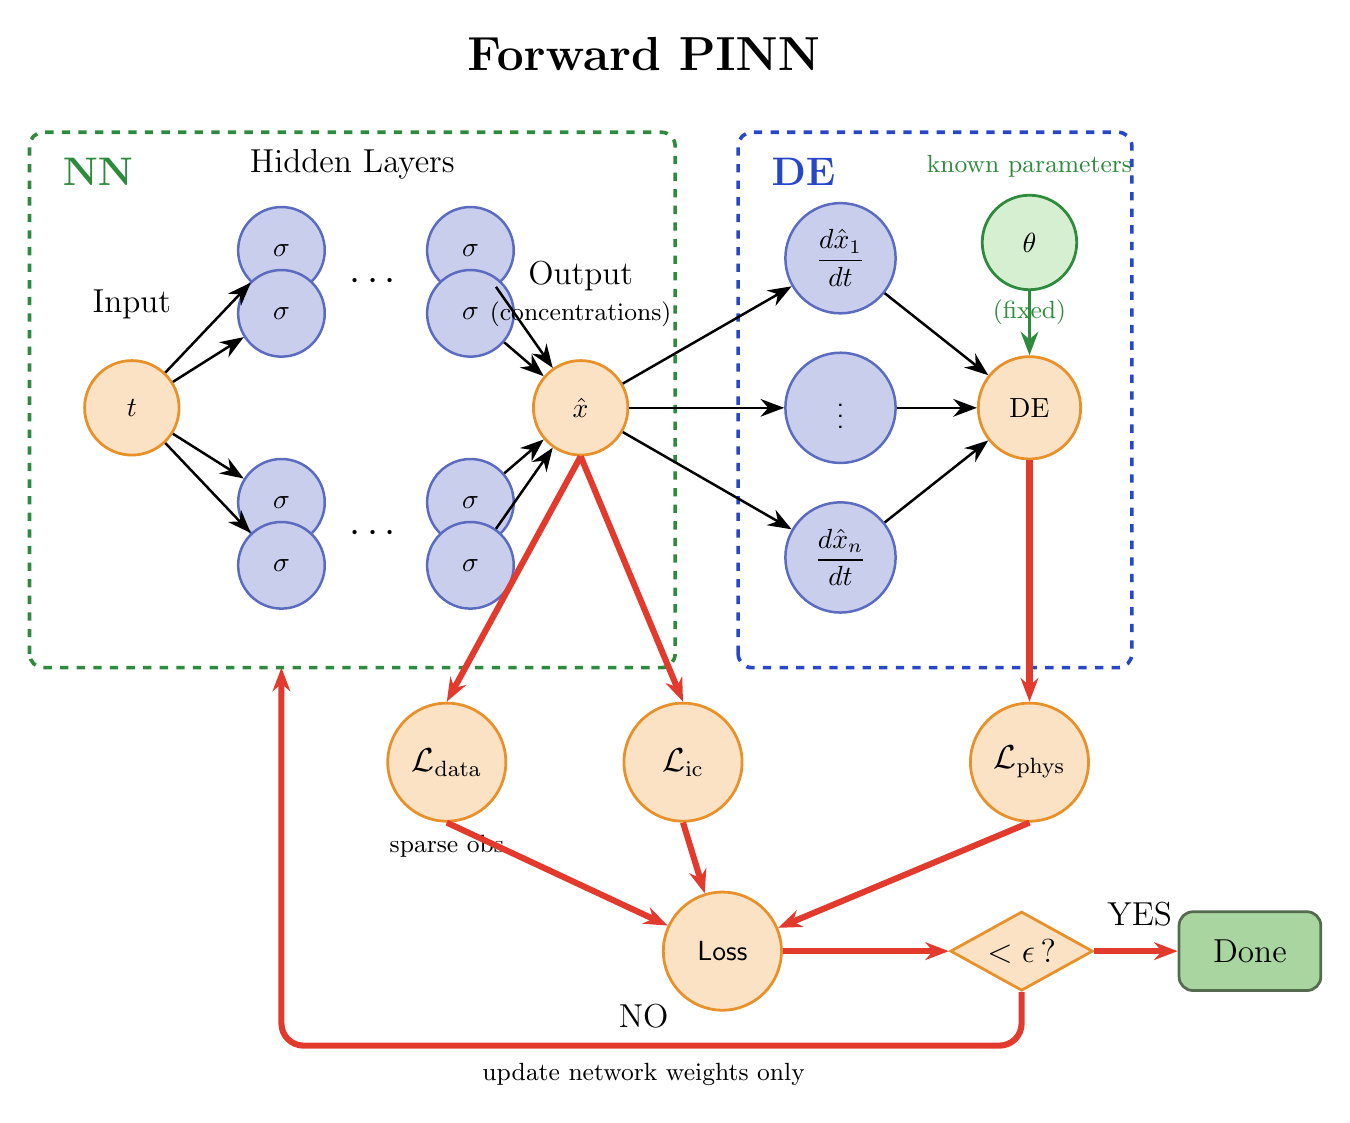
\begin{tikzpicture}[
    >={Stealth[length=3mm]},
    font=\sffamily,
    sig/.style={circle,draw=blueE,fill=blueF,line width=0.9pt,
                minimum size=11mm,inner sep=0pt},
    der/.style={circle,draw=blueE,fill=blueF,line width=0.9pt,
                minimum size=14mm,inner sep=0pt},
    orb/.style={circle,draw=orangeE,fill=orangeF,line width=1pt,inner sep=0pt},
    box/.style={dashed,line width=1.3pt,rounded corners=5pt},
    flow/.style={->,line width=0.9pt},
    loop/.style={->,line width=2.2pt,color=redLoop,rounded corners=8pt},
]

% =====================================================================
%  NN block
% =====================================================================
\draw[box,draw=greenBox] (0.2,1.4) rectangle (8.4,8.2);
\node[greenBox,font=\bfseries\Large,anchor=north west] at (0.5,8.0) {NN};
\node[font=\large,anchor=north] at (4.3,8.1) {Hidden Layers};

\node[font=\large,anchor=south] at (1.5,5.7) {Input};
\node[orb,minimum size=12mm] (tin) at (1.5,4.7) {$t$};

% two shown hidden layers (first and last); inner layers implied by dots
\foreach \y/\n in {6.7/a1,5.9/a2,3.5/a3,2.7/a4}
   \node[sig] (\n) at (3.4,\y) {$\sigma$};
\foreach \y/\n in {6.7/b1,5.9/b2,3.5/b3,2.7/b4}
   \node[sig] (\n) at (5.8,\y) {$\sigma$};
\node[font=\Large] at (4.6,6.3) {$\cdots$};
\node[font=\Large] at (4.6,3.1) {$\cdots$};

% the network output IS the unknown being solved for: the concentrations
\node[font=\large,anchor=south,align=center] at (7.2,5.6)
     {Output\\[-1pt]{\small(concentrations)}};
\node[orb,minimum size=12mm] (xhat) at (7.2,4.7) {$\hat{x}$};

% only the boundary connections are drawn (layers are fully connected,
% but the dense edges are omitted for clarity)
\foreach \n in {a1,a2,a3,a4} \draw[flow] (tin) -- (\n);
\foreach \n in {b1,b2,b3,b4} \draw[flow] (\n) -- (xhat);

% =====================================================================
%  DE block  (autodiff derivatives + ODE residual using the KNOWN theta)
% =====================================================================
\draw[box,draw=blueBox] (9.2,1.4) rectangle (14.2,8.2);
\node[blueBox,font=\bfseries\Large,anchor=north west] at (9.5,8.0) {DE};

\node[der] (d1) at (10.5,6.6) {$\dfrac{d\hat{x}_1}{dt}$};
\node[der] (dm) at (10.5,4.7) {$\vdots$};
\node[der] (dn) at (10.5,2.8) {$\dfrac{d\hat{x}_n}{dt}$};
\node[orb,minimum size=13mm] (de) at (12.9,4.7) {$\mathrm{DE}$};

% KNOWN ODE parameters (the forward element): fixed input, NOT recovered.
% Green = given/known, in contrast to the inverse diagram's purple unknown.
\node[circle,draw=knownE,fill=knownF,line width=1pt,minimum size=12mm]
     (theta) at (12.9,6.8) {$\theta$};
\node[knownE,font=\small,anchor=south] at (12.9,7.5) {known parameters};
\node[knownE,font=\small,anchor=north] at (12.9,6.2) {(fixed)};

\foreach \n in {d1,dm,dn} \draw[flow] (xhat) -- (\n);
\foreach \n in {d1,dm,dn} \draw[flow] (\n) -- (de);
\draw[flow,color=knownE,line width=1pt] (theta) -- (de);

% =====================================================================
%  Loss terms -> total Loss -> (< eps ?) -> Done / iterate
%  (compact cluster directly under the blocks)
% =====================================================================
\tikzset{lterm/.style={orb,minimum size=15mm,font=\large}}

% three loss components, sitting just below their sources
\node[lterm] (ldata) at (5.5,0.2)  {$\mathcal{L}_{\mathrm{data}}$};
\node[lterm] (lic)   at (8.5,0.2)  {$\mathcal{L}_{\mathrm{ic}}$};
\node[lterm] (lphys) at (12.9,0.2) {$\mathcal{L}_{\mathrm{phys}}$};
% forward = honest sparse-data hybrid: the data term is a handful of noisy obs
\node[font=\small,anchor=north] at (5.5,-0.6) {sparse obs};

% data fit + initial condition come from the network output;
% the physics residual comes from the DE node (straight down, no overlap)
\draw[loop] (xhat.south) -- (ldata.north);
\draw[loop] (xhat.south) -- (lic.north);
\draw[loop] (de.south)   -- (lphys.north);

% total loss = sum of the three terms
\node[orb,minimum size=15mm] (loss) at (9.0,-2.2) {Loss};
\foreach \n in {ldata,lic,lphys} \draw[loop] (\n.south) -- (loss);

% convergence check
\node[diamond,draw=orangeE,fill=orangeF,line width=1pt,aspect=1.8,
      inner sep=2pt,font=\large] (eps) at (12.8,-2.2) {$<\epsilon\,?$};
\draw[loop] (loss.east) -- (eps.west);

% Done
\node[rounded corners=5pt,draw=doneG!50!black,fill=doneG,line width=1pt,
      minimum width=1.8cm,minimum height=1.0cm,font=\large] (done)
      at (15.7,-2.2) {Done};
\draw[loop] (eps.east) -- (done.west);
\node[font=\large,anchor=south] at (14.3,-2.0) {YES};

% NO -> iterate back into the NN block.  In the forward problem the loop
% updates ONLY the network weights; theta stays fixed.
\draw[loop] (eps.south) -- (12.8,-3.4) -- (3.4,-3.4) -- (3.4,1.4);
\node[font=\large,anchor=south] at (8.0,-3.3) {NO};
\node[font=\small,anchor=north] at (8.0,-3.5) {update network weights only};

% =====================================================================
%  Title
% =====================================================================
\node[font=\bfseries\LARGE] at (8.0,9.2) {Forward PINN};

\end{tikzpicture}
\end{document}
